% Preámbulo
\documentclass[stu, 12pt, letterpaper, donotrepeattitle, floatsintext, natbib]{apa7}
\usepackage[utf8]{inputenc}
\usepackage{comment}
\usepackage{marvosym}
\usepackage{graphicx}
\usepackage{float}
\usepackage{amsmath}
\usepackage[normalem]{ulem}
\usepackage[spanish]{babel} 
\usepackage{indentfirst} %para le formato que quiere la profe QUITAR SI QUIERES OG APA7
\usepackage{ragged2e} %para le formato que quiere la profe QUITAR SI QUIERES OG APA7
\usepackage{indentfirst} %para le formato que quiere la profe QUITAR SI QUIERES OG APA7
\usepackage{multirow,booktabs,setspace,caption} %formato de figuras APA
\DeclareCaptionLabelSeparator*{spaced}{\\[2ex]}
\DeclareCaptionLabelSeparator*{spaced}{\\[2ex]}
\captionsetup[figure]{textfont=it,format=plain,justification=justified,
  singlelinecheck=false,labelsep=spaced,skip=0pt}

\selectlanguage{spanish}
\useunder{\uline}{\ul}{}
\newcommand{\myparagraph}[1]{\paragraph{#1}\mbox{}\\}

% Portada
%\thispagestyle{empty}
\title{\Large Tarea 2 Unidad 4: Tipos de texturas en una imágen}
\author{Abraham Jhared Flores Azcona} % (autores separados, consultar al docente)
% Manera oficial de colocar los autores:
%\author{Autor(a) I, Autor(a) II, Autor(a) III, Autor(a) X}
\affiliation{Instituto Tecnológico de Tijuana}
\course{SCC-1010SC5C: Graficación}
\professor{Dra. Martha Elena Pulido}
\duedate{20 de septiembre de 2021}

\begin{document}
    % Índices
    \pagenumbering{arabic}
    \maketitle

    % Contenido
    \renewcommand\contentsname{Contenido}
    \tableofcontents
    \renewcommand{\listfigurename}{Figuras}
    \listoffigures

    % Cuerpo 
    %NOTA: PARA CITAR ESTILO "Merts (2003)" usar \cite{<nombre_cita_bib>}
    %    
    \newpage
    \section{Típos}
    Son \begin{justifying}
      también conocidos como mapas de texturas. A grandes rasgos encontramos los siguientes:
      de color, bump, displacement, reflection, gloss, metalness, AO, Albedo y Fuzz \citep{barber-no-date}.
    \end{justifying}
    \vspace{\baselineskip}
    \subsection{Color}
    Simplemente \begin{justifying}
      es una foto que tendríamos si esta se tomase enfrente del material y se toma dicha foto.\par
    \end{justifying}
    \begin{figure}[H]
      \caption{\emph{Ejemplo de textura de color.}}
      \centering
      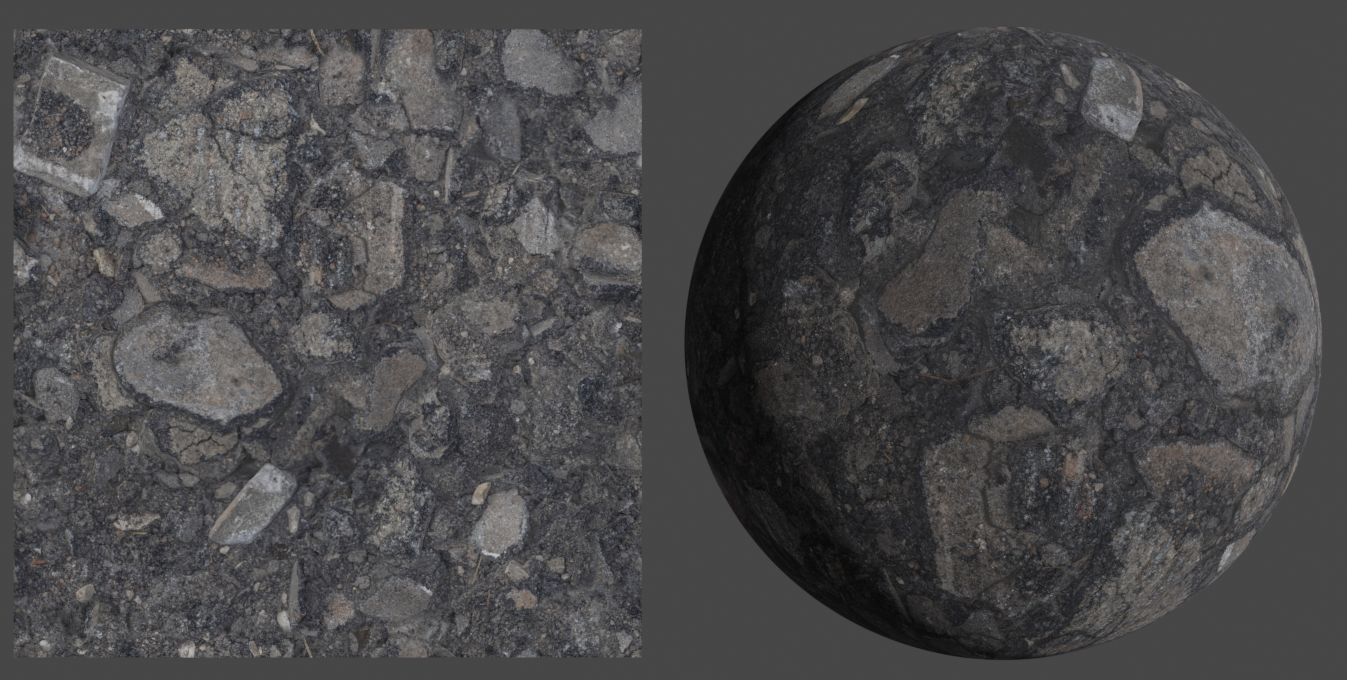
\includegraphics[width=10cm,height=6cm]{color.png}
      \bigskip
    \end{figure}
    \subsection{Bump}
    Es \begin{justifying}
      aquel conocido como el infame mapa púrpura. Cada color representa una dirección distinta en los ejes, permitiendo a la computadora
      entender fácilmente a la figura.\par
    \end{justifying}
    \begin{figure}[H]
      \caption{\emph{Ejemplo de textura Bump.}}
      \centering
      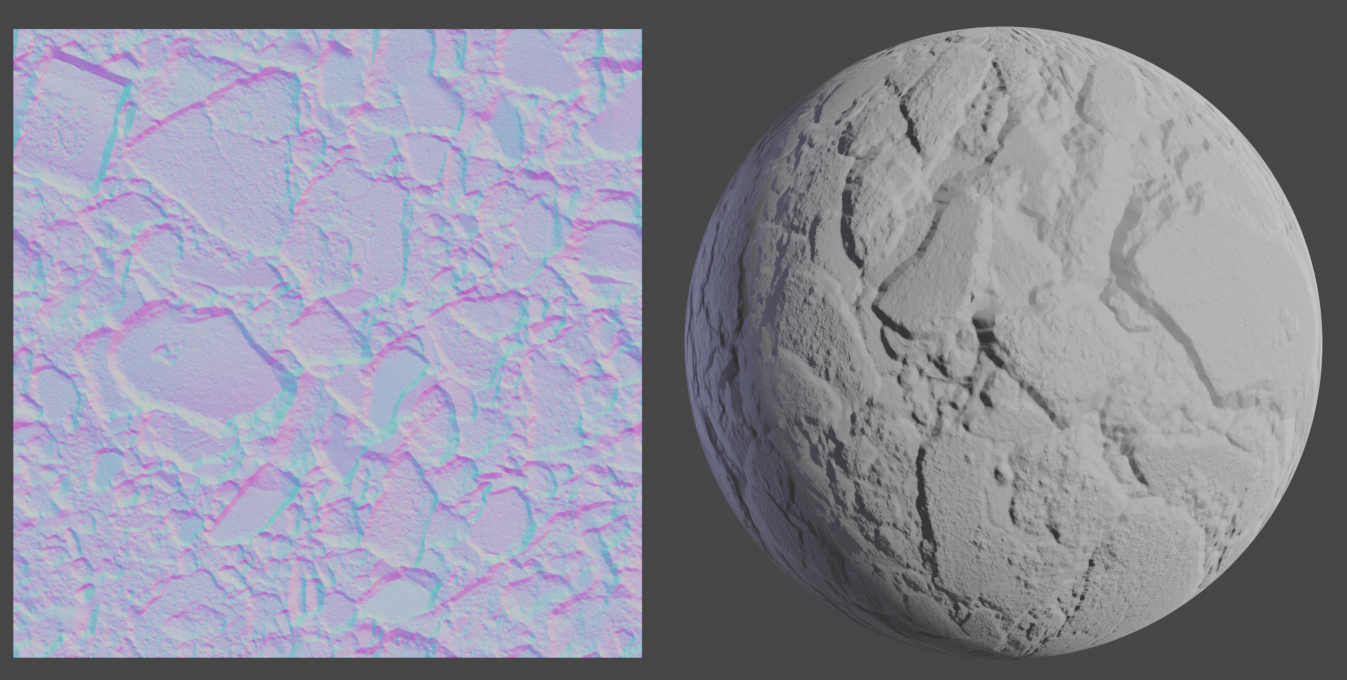
\includegraphics[width=10cm,height=6cm]{normals.png}
      \bigskip
    \end{figure}
    \subsection{Displacement}
    Se \begin{justifying}
      llaman así debido a que desplazan físicamente el mesh en el cual son aplicados. Se pueden crear a partir de un modelo de alta resolución
    o pintado a mano \citep{pluralsight-2014}.\par
    \end{justifying}
    \begin{figure}[H]
      \caption{\emph{Ejemplo de textura Displacement.}}
      \centering
      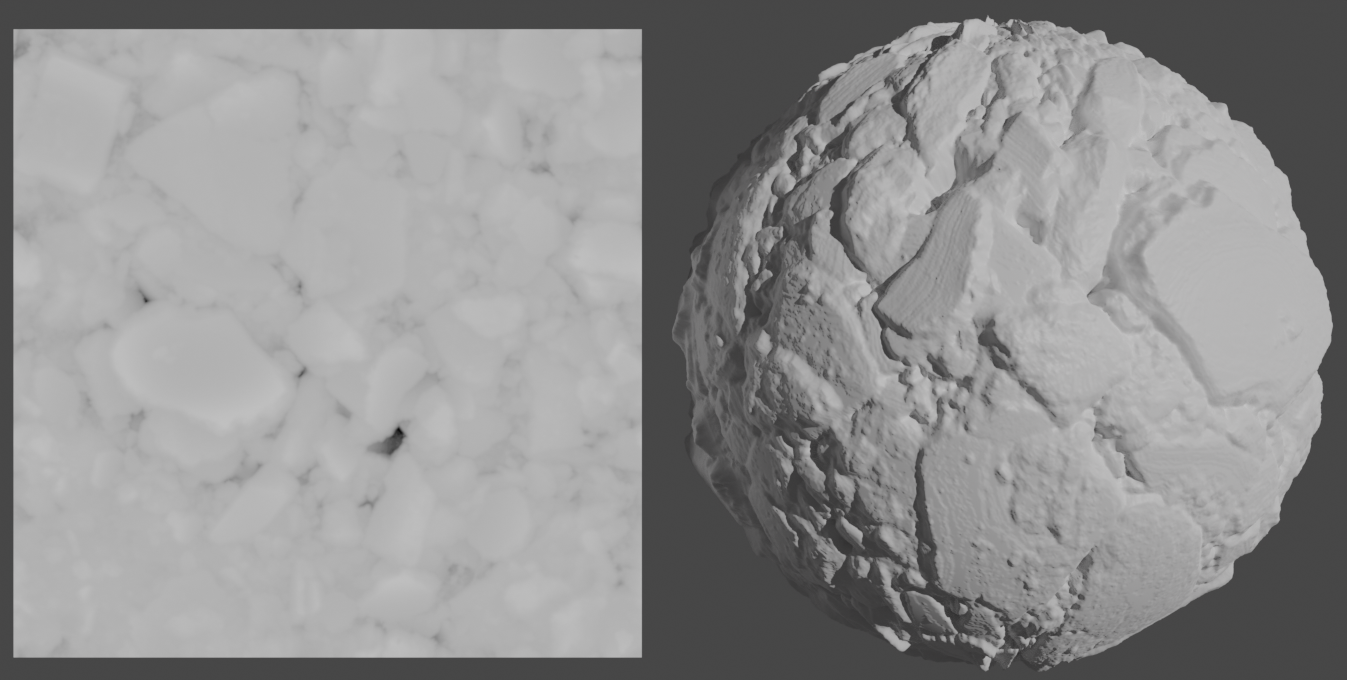
\includegraphics[width=10cm,height=6cm]{displacement.png}
      \bigskip
    \end{figure}
    \subsection{Reflection}
    Muy \begin{justifying}
      útil para reducit recursos en ray tracing. Genearlmente se considera al objeto a graficar dicha textura en el centro de una gran esfera, donde 
      el entorno se proyecta. Este mapeo usa un mapa de latitud-longitud indizado por el rayo reflejado.
    \end{justifying}
    \begin{figure}[H]
      \caption{\emph{Ejemplo de textura Reflection.}}
      \centering
      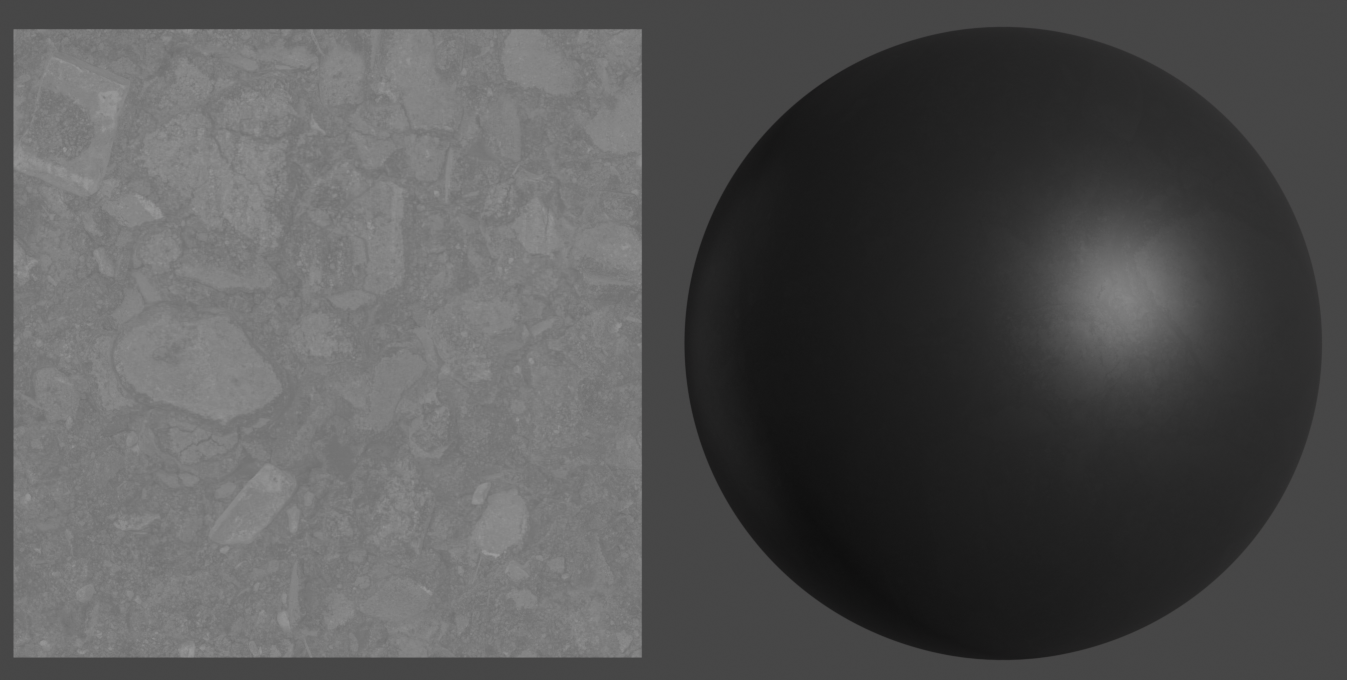
\includegraphics[width=10cm,height=6cm]{reflection.png}
      \bigskip
    \end{figure}
    \subsection{Gloss}
    Usa \begin{justifying}
      shaders PBR. Este controla la agresividad de las reflecciones, dando una textura similar a los rastros de las pistas de patinaje sobre hielo \citep{unknown-author-no-date}.\par
    \end{justifying}
    \begin{figure}[H]
      \caption{\emph{Ejemplo de textura Gloss.}}
      \centering
      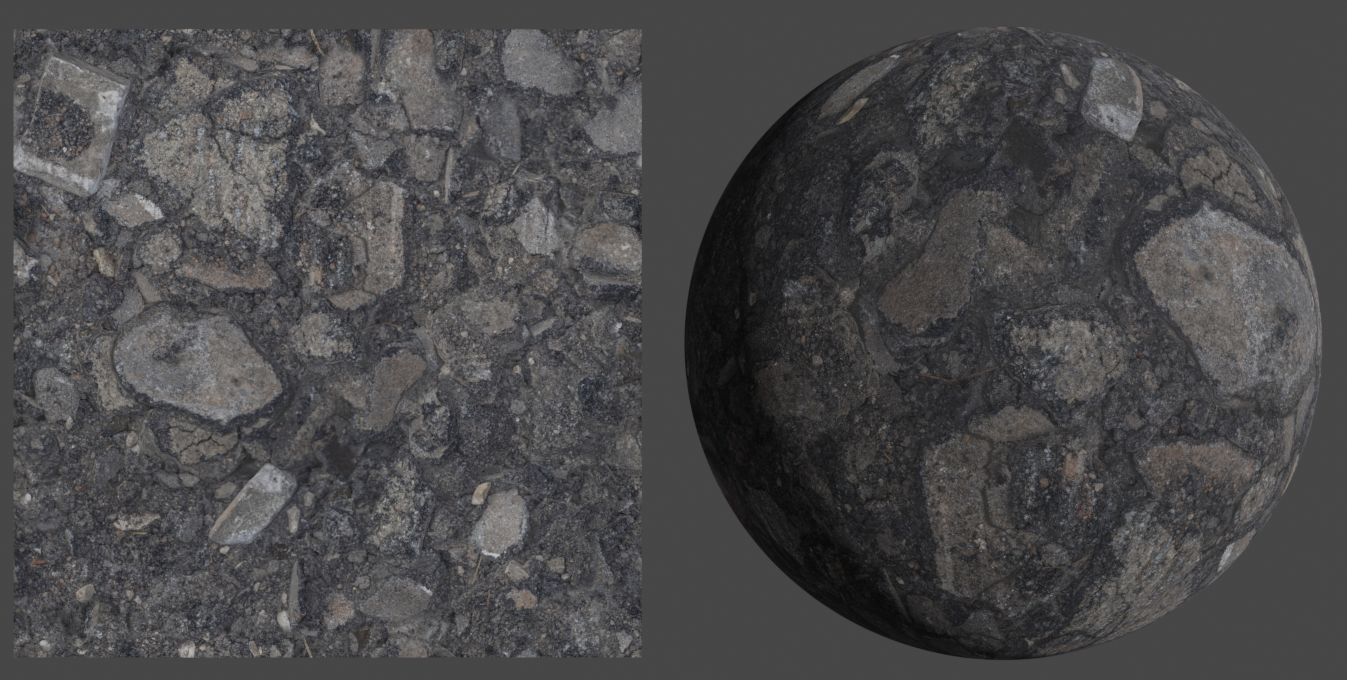
\includegraphics[width=10cm,height=6cm]{color.png}
      \bigskip
    \end{figure}
    \subsection{Metalness}
    Se \begin{justifying}
      le indica al programa que parte del objeto renderizar como metal y cual nó para poder apicar las propiedades de reflección
      de un metal.\par
    \end{justifying}
    \begin{figure}[H]
      \caption{\emph{Ejemplo de textura Metalness}}
      \centering
      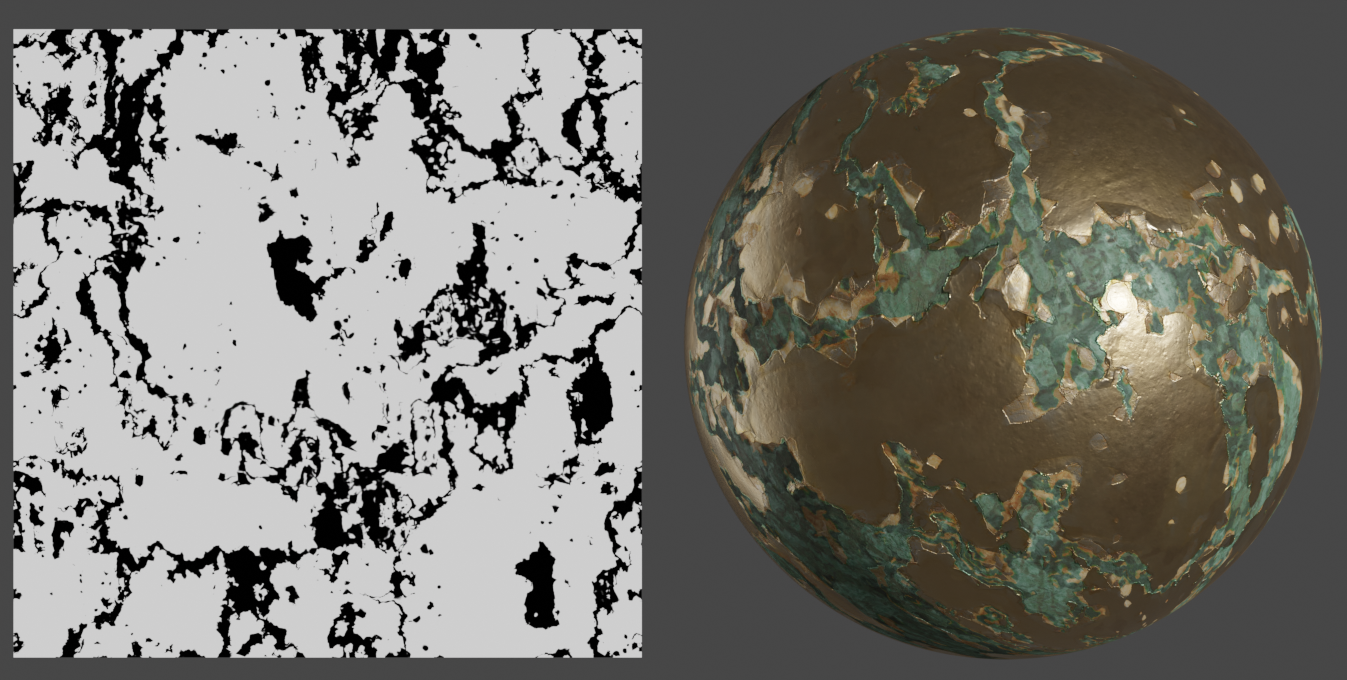
\includegraphics[width=10cm,height=6cm]{metalness.png}
      \bigskip
    \end{figure}
    \subsection{AO}
    Un \begin{justifying}
      mapeo que permite tener más sombras. Permite dar más detalles y más sombras.\par
    \end{justifying}
    \begin{figure}[H]
      \caption{\emph{Ejemplo de textura AO}}
      \centering
      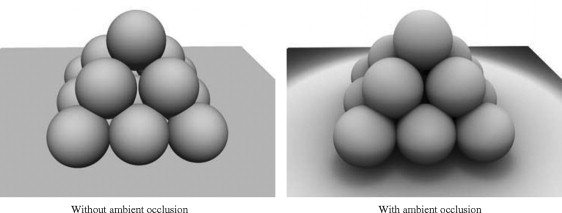
\includegraphics[width=10cm,height=6cm]{ao.jpg}
      \bigskip
    \end{figure}
    
    \newpage   
    % Referencias
    \renewcommand\refname{\textbf{Referencias}}
    \bibliography{referencias}
    
\end{document}